\begin{figure*}[ht!]
	\captionsetup[subfigure]{justification=centering}
	\centering
	\begin{subfigure}[t]{0.5\textwidth}
		\centering
		
\includegraphics[width=\linewidth]{protocol-charts-cios}
		\caption{Construction stage number of \acrshort{io} requests}%
		\label{figure:protocols-ios:c}
	\end{subfigure}%
	~ % chktex 39
	\begin{subfigure}[t]{0.5\textwidth}
		\centering
		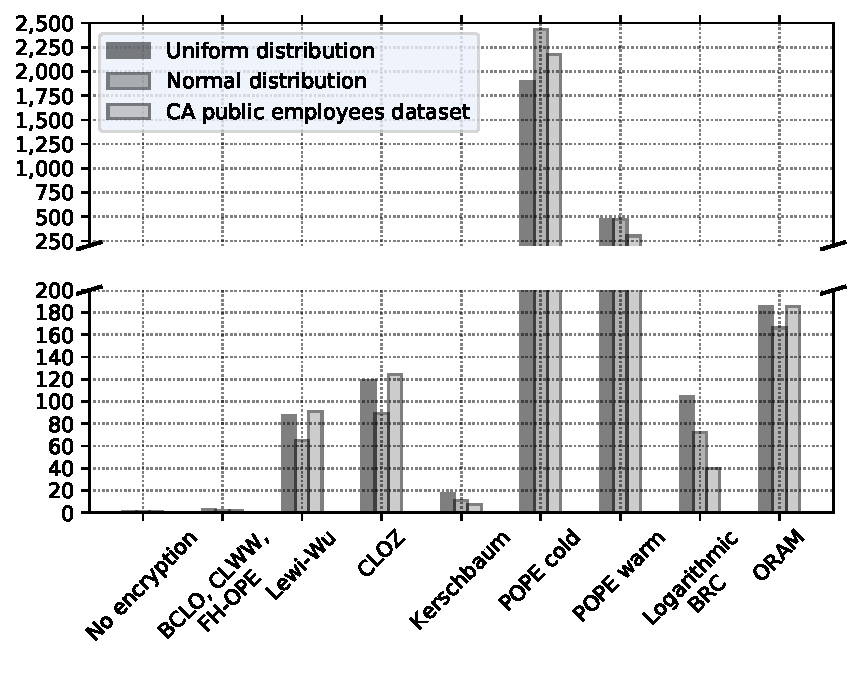
\includegraphics[width=\linewidth]{protocol-charts-qios}
		\caption{Queries stage number of \acrshort{io} requests}%
		\label{figure:protocols-ios:q}
	\end{subfigure}%
	\caption{Number of \acrshort{io} requests for different protocols and data distributions}%
	\label{figure:protocols-ios}
\end{figure*}

\begin{figure*}[ht!]
	\captionsetup[subfigure]{justification=centering}
	\centering
	\begin{subfigure}[t]{0.5\textwidth}
		\centering
		
\includegraphics[width=\linewidth]{protocol-charts-csize}
		\caption{Construction stage communication size (bytes transferred)}%
		\label{figure:protocols-size:c}
	\end{subfigure}%
	~ % chktex 39
	\begin{subfigure}[t]{0.5\textwidth}
		\centering
		
\includegraphics[width=\linewidth]{protocol-charts-qsize}
		\caption{Queries stage communication size (transferred bytes, log scale)}%
		\label{figure:protocols-size:q}
	\end{subfigure}%
	\caption{Communication size for different protocols and data distributions}%
	\label{figure:protocols-size}
\end{figure*}

\begin{figure*}[ht!]
	\captionsetup[subfigure]{justification=centering}
	\centering
	\begin{subfigure}[t]{0.5\textwidth}
		\centering
		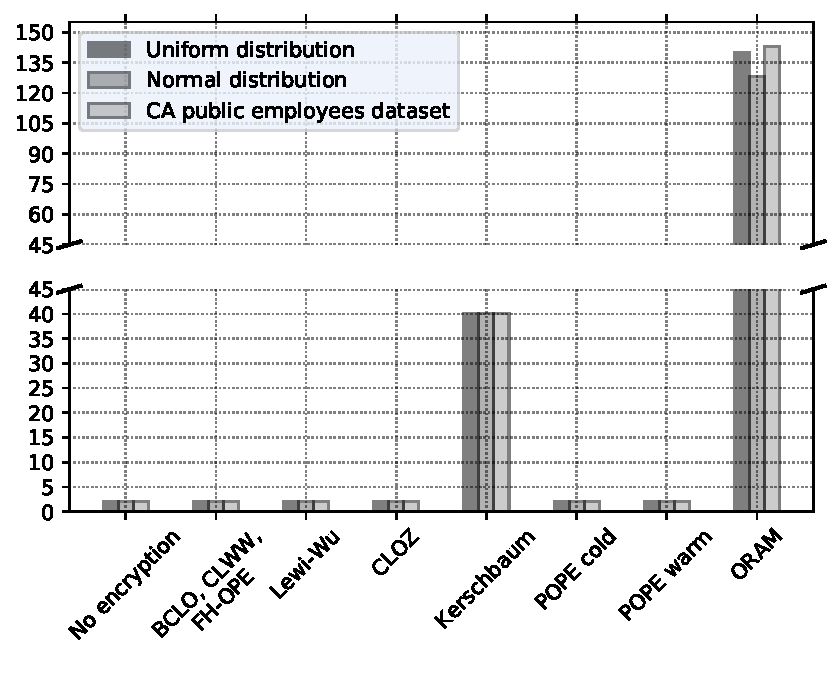
\includegraphics[width=\linewidth]{protocol-charts-cvol}
		\caption{Construction stage communication volume (number of messages)}%
		\label{figure:protocols-vol:c}
	\end{subfigure}%
	~ % chktex 39
	\begin{subfigure}[t]{0.5\textwidth}
		\centering
		
\includegraphics[width=\linewidth]{protocol-charts-qvol}
		\caption{Queries stage communication volume (number of messages)}%
		\label{figure:protocols-vol:q}
	\end{subfigure}%
	\caption{Communication volume for different protocols and data distributions}%
	\label{figure:protocols-vol}
\end{figure*}
